\chapter{Supplemental material for \chapref{chap:mer130}}
\label{chap:mer130Suppl}

\section{Supplemental Figures}

\begin{figure}[htbp]
\centering
\begin{tabular}{l}
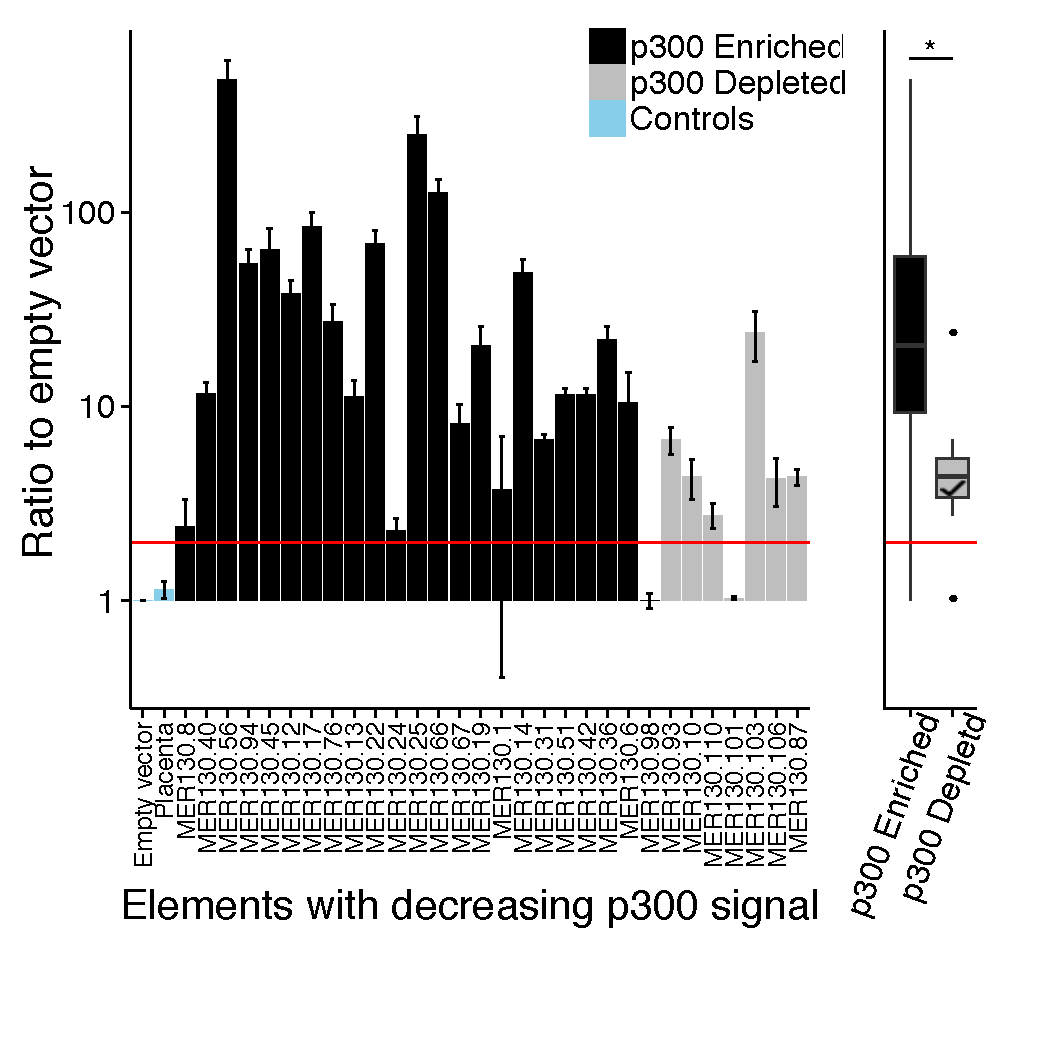
\epsfig{file=figures/mer130FigureS1.pdf,width=0.7\linewidth,clip=,trim=0 0 0 0} \\
\end{tabular}
\caption[MER130 instances function as enhancers in dissociated cortical neurons]{
{\bf MER130 instances function as enhancers in dissociated cortical neurons.}
Average fold activity when transfected
in dissociated cortical neurons relative to the empty vector. MER130
elements sorted in order of decreasing maximum p300 ChIP-seq intensity.
MER130 elements enriched for the p300 signal in black (\emph{n} = 23)
and depleted for the p300 signal in gray (\emph{n} = 7). Error bars
represent standard deviations. \emph{n} = 3 biological replicates x 3
technical replicates for each condition. t-test. *\emph{p}-value \textless{}
0.05.
}
\label{fig:mer130FigS1}
\end{figure}

\begin{figure}[htbp]
\centering
\begin{tabular}{l}

\epsfig{file=figures/mer130FigureS2.pdf,width=0.99\linewidth,clip=,trim=0 0 0 0} \\
\end{tabular}
\caption[MER130 multiple alignment]{
{\bf MER130 multiple alignment.}
A multiple alignment of all 107 MER130
instances, virtually all of which preserve the 5 binding site core.
}
\label{fig:mer130FigS2}
\end{figure}

\begin{figure}[htbp]
\centering
\begin{tabular}{l}
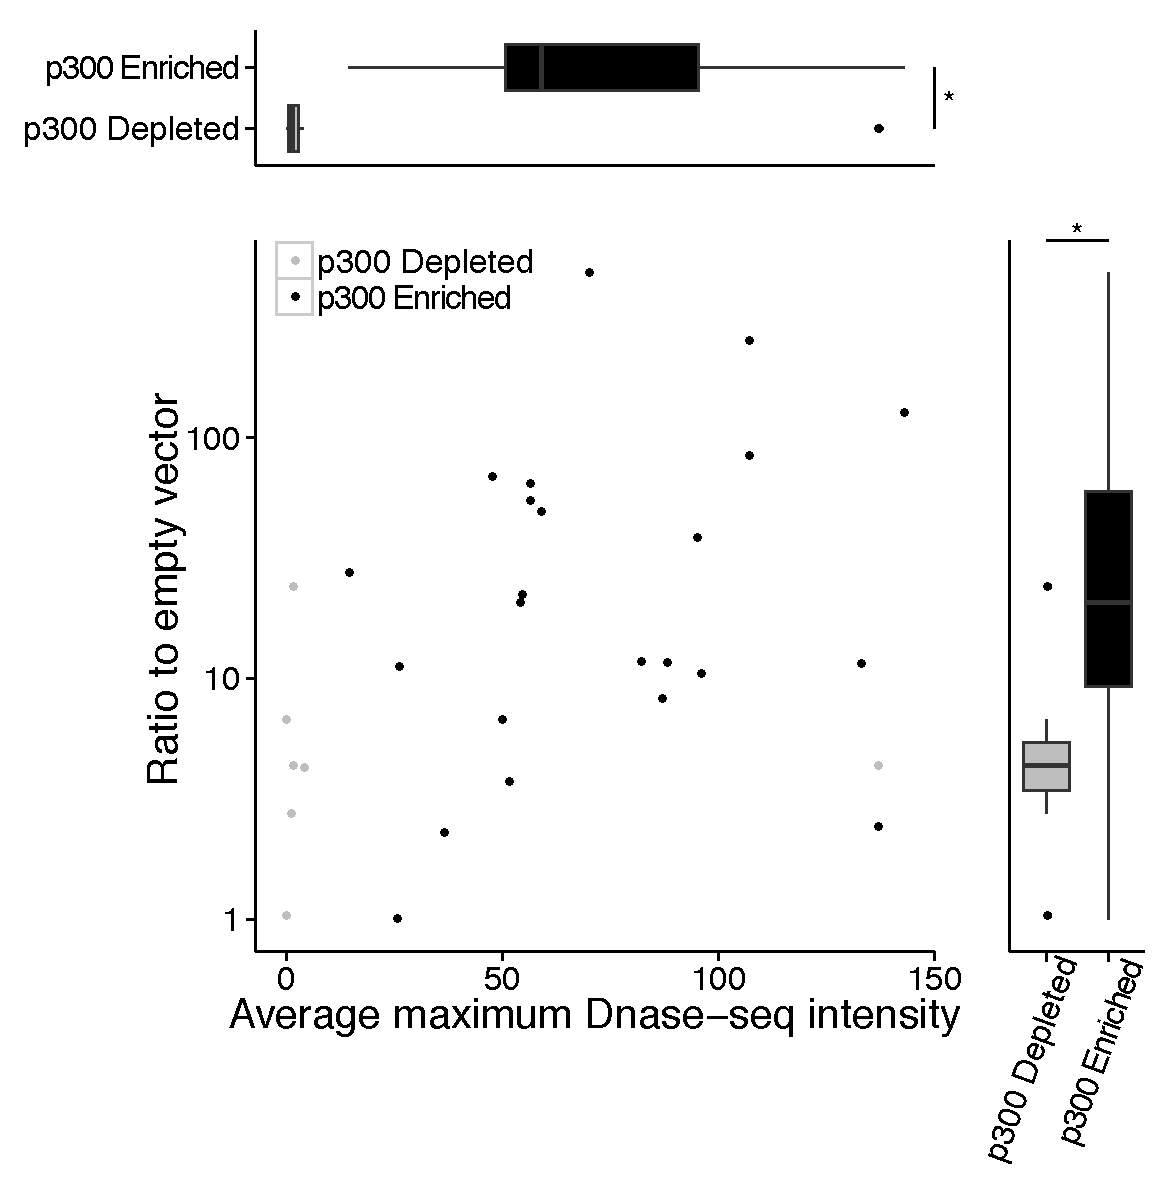
\epsfig{file=figures/mer130FigureS3.pdf,width=0.7\linewidth,clip=,trim=0 0 0 0} \\
\end{tabular}
\caption[DNase-seq intensity vs. transfection activity]{
{\bf DNase-seq intensity vs. transfection activity.}
Average DNase-seq intensity across day
85 human fetal brain tissue replicates (x-axis) plotted against average
fold activity relative to the empty vector (y-axis) for the same set of
MER130 instances transfected into dissociated cortical neurons. MER130
elements enriched for the p300 signal in black (\emph{n} = 23) and
depleted for the p300 signal in gray (\emph{n =} 7). t-test. *\emph{p}-value
\textless{} 0.05.
}
\label{fig:mer130FigS3}
\end{figure}

\section{Supplemental Tables}

\begin{center}
\begin{longtable}{@{}p{0.25\linewidth}p{0.2\linewidth}p{0.2\linewidth}p{0.2\linewidth}@{}}
\caption[MER130 instances in mouse]{{\bf MER130 instances in mouse.}
Identified by nhmmer (see Methods in \ref{sec:mer130Methods}) in the NCBI37/mm9 mouse assembly.
}
\label{tab:mer130TabS1} \\

\hline \textbf{mm9 chromosome} & \textbf{Start position} & \textbf{End position} & \textbf{Name} \\ \hline 
\endfirsthead

\hline \textbf{mm9 chromosome} & \textbf{Start position} & \textbf{End
position} & \textbf{Name} \\ \hline 
\endhead

\hline
\endlastfoot

chr3 & 149213528 & 149213837 & MER130.1\tabularnewline
chr15 & 42592816 & 42592880 & MER130.2\tabularnewline
chr1 & 192390632 & 192390976 & MER130.3\tabularnewline
chr10 & 111373706 & 111374076 & MER130.4\tabularnewline
chr12 & 93273917 & 93274100 & MER130.5\tabularnewline
chr16 & 82661316 & 82661607 & MER130.6\tabularnewline
chr5 & 59366593 & 59366899 & MER130.7\tabularnewline
chr10 & 91182667 & 91183115 & MER130.8\tabularnewline
chr2 & 6960107 & 6960257 & MER130.9\tabularnewline
chr5 & 76389906 & 76390041 & MER130.10\tabularnewline
chrX & 66281974 & 66282187 & MER130.11\tabularnewline
chr14 & 123357211 & 123357465 & MER130.12\tabularnewline
chr16 & 72088406 & 72088618 & MER130.13\tabularnewline
chr11 & 26486760 & 26487197 & MER130.14\tabularnewline
chr17 & 78850810 & 78851192 & MER130.15\tabularnewline
chr4 & 21475030 & 21475324 & MER130.16\tabularnewline
chr2 & 73770833 & 73771101 & MER130.17\tabularnewline
chr16 & 72585559 & 72585799 & MER130.18\tabularnewline
chr15 & 31919395 & 31919637 & MER130.19\tabularnewline
chr3 & 85197458 & 85197660 & MER130.20\tabularnewline
chr6 & 5906456 & 5906821 & MER130.21\tabularnewline
chr1 & 32520019 & 32520321 & MER130.22\tabularnewline
chr10 & 121383312 & 121383550 & MER130.23\tabularnewline
chr6 & 16907063 & 16907326 & MER130.24\tabularnewline
chr12 & 107258342 & 107258648 & MER130.25\tabularnewline
chr8 & 52773395 & 52773689 & MER130.26\tabularnewline
chr8 & 17465577 & 17465815 & MER130.27\tabularnewline
chr2 & 63948029 & 63948206 & MER130.28\tabularnewline
chr19 & 49153411 & 49153517 & MER130.29\tabularnewline
chr19 & 51802258 & 51802437 & MER130.30\tabularnewline
chr13 & 48123239 & 48123471 & MER130.31\tabularnewline
chr2 & 82213354 & 82213558 & MER130.32\tabularnewline
chr8 & 90169311 & 90169558 & MER130.33\tabularnewline
chr2 & 78185663 & 78185879 & MER130.34\tabularnewline
chr18 & 64598088 & 64598213 & MER130.35\tabularnewline
chr2 & 57759274 & 57759618 & MER130.36\tabularnewline
chr17 & 78303759 & 78304034 & MER130.37\tabularnewline
chr3 & 68157491 & 68157731 & MER130.38\tabularnewline
chr9 & 74166728 & 74166824 & MER130.39\tabularnewline
chr8 & 90199467 & 90199632 & MER130.40\tabularnewline
chr4 & 94106030 & 94106148 & MER130.41\tabularnewline
chr2 & 43672783 & 43673121 & MER130.42\tabularnewline
chr2 & 56085573 & 56085764 & MER130.43\tabularnewline
chr16 & 28761888 & 28761997 & MER130.44\tabularnewline
chr2 & 18556785 & 18556976 & MER130.45\tabularnewline
chr1 & 183952006 & 183952301 & MER130.47\tabularnewline
chr15 & 40900331 & 40900526 & MER130.48\tabularnewline
chr1 & 78050307 & 78050636 & MER130.49\tabularnewline
chr12 & 47472759 & 47473058 & MER130.50\tabularnewline
chr12 & 39028085 & 39028340 & MER130.51\tabularnewline
chr12 & 50030097 & 50030315 & MER130.52\tabularnewline
chr11 & 18387979 & 18388084 & MER130.53\tabularnewline
chr18 & 23505773 & 23505886 & MER130.54\tabularnewline
chr5 & 60668031 & 60668304 & MER130.55\tabularnewline
chr13 & 95145888 & 95146198 & MER130.56\tabularnewline
chr12 & 54713097 & 54713392 & MER130.57\tabularnewline
chr1 & 139743927 & 139744144 & MER130.58\tabularnewline
chr10 & 54469112 & 54469302 & MER130.59\tabularnewline
chr17 & 11669081 & 11669223 & MER130.60\tabularnewline
chrX & 143163220 & 143163378 & MER130.61\tabularnewline
chr11 & 19162882 & 19163203 & MER130.62\tabularnewline
chr4 & 99232256 & 99232380 & MER130.63\tabularnewline
chr6 & 111689190 & 111689279 & MER130.64\tabularnewline
chr7 & 140680006 & 140680246 & MER130.65\tabularnewline
chr2 & 50510542 & 50510637 & MER130.66\tabularnewline
chr6 & 100077946 & 100078114 & MER130.67\tabularnewline
chr6 & 19165247 & 19165397 & MER130.68\tabularnewline
chr12 & 27803589 & 27803695 & MER130.69\tabularnewline
chr6 & 6743998 & 6744232 & MER130.70\tabularnewline
chr7 & 58670946 & 58671173 & MER130.71\tabularnewline
chr1 & 48333229 & 48333326 & MER130.72\tabularnewline
chr15 & 35198547 & 35198786 & MER130.73\tabularnewline
chr4 & 82591594 & 82591793 & MER130.74\tabularnewline
chr7 & 36518733 & 36518948 & MER130.76\tabularnewline
chr15 & 22656438 & 22656591 & MER130.77\tabularnewline
chr9 & 47115318 & 47115455 & MER130.78\tabularnewline
chr7 & 72250084 & 72250179 & MER130.79\tabularnewline
chr9 & 105425505 & 105425645 & MER130.80\tabularnewline
chr12 & 39764820 & 39764975 & MER130.81\tabularnewline
chr10 & 116036701 & 116036794 & MER130.82\tabularnewline
chr12 & 37018024 & 37018167 & MER130.83\tabularnewline
chr8 & 54933223 & 54933464 & MER130.84\tabularnewline
chr1 & 148548001 & 148548049 & MER130.85\tabularnewline
chr9 & 30232922 & 30233018 & MER130.86\tabularnewline
chr16 & 83768718 & 83768845 & MER130.87\tabularnewline
chr5 & 106422248 & 106422376 & MER130.88\tabularnewline
chr12 & 12627126 & 12627374 & MER130.89\tabularnewline
chr18 & 17545739 & 17545816 & MER130.90\tabularnewline
chr10 & 51513821 & 51513991 & MER130.91\tabularnewline
chr4 & 82509395 & 82509591 & MER130.92\tabularnewline
chr6 & 19565949 & 19566025 & MER130.93\tabularnewline
chr11 & 91288193 & 91288316 & MER130.94\tabularnewline
chrX & 89586430 & 89586499 & MER130.95\tabularnewline
chr6 & 19845744 & 19845848 & MER130.96\tabularnewline
chr6 & 33048942 & 33049049 & MER130.97\tabularnewline
chr8 & 92938136 & 92938253 & MER130.98\tabularnewline
chr9 & 70057275 & 70057401 & MER130.99\tabularnewline
chr10 & 63593293 & 63593541 & MER130.100\tabularnewline
chr11 & 83419419 & 83419565 & MER130.101\tabularnewline
chr15 & 63001904 & 63002059 & MER130.102\tabularnewline
chr13 & 56044847 & 56045004 & MER130.103\tabularnewline
chr4 & 62294274 & 62294379 & MER130.105\tabularnewline
chr7 & 38134116 & 38134266 & MER130.106\tabularnewline
chr14 & 84434751 & 84434844 & MER130.107\tabularnewline
chr10 & 114109092 & 114109219 & MER130.109\tabularnewline
chr10 & 18152254 & 18152359 & MER130.110\tabularnewline
chr8 & 6533117 & 6533211 & MER130.112\tabularnewline
\end{longtable}
\end{center}

\begin{center}
\begin{longtable}{@{}p{0.17\linewidth}p{0.12\linewidth}p{0.15\linewidth}p{0.2\linewidth}p{0.2\linewidth}@{}}
\caption[Repeat densities observed in 75 vertebrate genome drafts from UCSC and Genbank]{{\bf Repeat densities observed in 75 vertebrate genome drafts from UCSC and Genbank.}
Repeat occurrences and repeat density observed in each vertebrate genome
}
\label{tab:mer130TabS2} \\

\hline \textbf{Common name} & \textbf{Genome assembly} & \textbf{MER130 instances} & \textbf{Genome or scaffold size} & \textbf{Repeat density (copies / Mb)} \\ \hline 
\endfirsthead

\hline \textbf{Common name} & \textbf{Genome assembly} & \textbf{MER130 instances} & \textbf{Genome or scaffold size} & \textbf{Repeat density (copies / Mb)} \\ \hline 
\endhead

\hline
\endlastfoot

Green sea turtle & Scaffold & 1124 & 2,208,393,880 &
0.508967178\tabularnewline
Painted turtle & chrPic1 & 1067 & 2,589,745,704 &
0.412009565\tabularnewline
Rock dove & Scaffold & 359 & 1,107,971,856 & 0.32401545\tabularnewline
Spiny softshell turtle & Scaffold & 621 & 1,931,078,847 &
0.321581898\tabularnewline
Saker falcon & Scaffold & 377 & 1,174,811,715 &
0.320902486\tabularnewline
Peregrine falcon & Scaffold & 375 & 1,171,955,363 &
0.319978057\tabularnewline
Duck & Scaffold & 340 & 1,105,035,747 & 0.307682354\tabularnewline
Budgerigar & melUnd1 & 331 & 1,117,373,619 & 0.296230369\tabularnewline
Chicken & galGal4 & 297 & 1,046,932,099 & 0.28368602\tabularnewline
American alligator & allMis1 & 616 & 2,174,259,888 &
0.283314798\tabularnewline
Scarlet macaw & Scaffold & 334 & 1,204,683,257 &
0.277251301\tabularnewline
Chinese soft shelled turtle & Scaffold & 608 & 2,202,466,388 &
0.276054156\tabularnewline
Turkey & melGal1 & 283 & 1,061,817,101 & 0.266524244\tabularnewline
Medium Ground Finch & geoFor1 & 283 & 1,065,292,181 &
0.265654818\tabularnewline
Medium ground finch & Scaffold & 283 & 1,065,292,181 &
0.265654818\tabularnewline
Ground tit & Scaffold & 277 & 1,042,980,823 & 0.265584941\tabularnewline
Zebra Finch & taeGut1 & 319 & 1,233,186,341 & 0.258679479\tabularnewline
White-throated sparrow & Scaffold & 267 & 1,052,600,561 &
0.253657475\tabularnewline
Platypus & ornAna1 & 224 & 1,996,811,212 & 0.112178857\tabularnewline
Lizard & anoCar2 & 141 & 1,799,143,587 & 0.078370621\tabularnewline
White rhinoceros & cerSim1 & 192 & 2,464,367,180 &
0.077910468\tabularnewline
Horse & equCab2 & 191 & 2,484,532,062 & 0.076875643\tabularnewline
Panda & ailMel1 & 168 & 2,299,509,015 & 0.073059074\tabularnewline
Alpaca & vicPac2 & 158 & 2,172,177,994 & 0.072738054\tabularnewline
Megabat & pteVam1 & 140 & 1,996,076,410 & 0.070137596\tabularnewline
Microbat & myoLuc2 & 141 & 2,034,575,300 & 0.069301932\tabularnewline
Cat & felCat5 & 169 & 2,455,541,136 & 0.068823934\tabularnewline
Dog & canFam3 & 164 & 2,410,976,875 & 0.06802222\tabularnewline
Bushbaby & otoGar3 & 167 & 2,519,724,550 & 0.066277086\tabularnewline
Tasmanian devil & sarHar1 & 206 & 3,174,693,010 &
0.064888164\tabularnewline
Opossum & monDom5 & 232 & 3,605,631,728 & 0.064343787\tabularnewline
Ferret & musFur1 & 155 & 2,410,758,013 & 0.06429513\tabularnewline
Dolphin & turTru2 & 164 & 2,551,996,573 & 0.064263409\tabularnewline
Squirrel monkey & saiBol1 & 166 & 2,608,572,064 &
0.063636348\tabularnewline
Squirrel & speTri2 & 155 & 2,478,393,770 & 0.062540506\tabularnewline
Manatee & triMan1 & 191 & 3,103,808,406 & 0.061537304\tabularnewline
Baboon & papAnu2 & 178 & 2,948,380,710 & 0.060372122\tabularnewline
Rhesus & rheMac3 & 179 & 2,969,988,180 & 0.0602696\tabularnewline
Gibbon & nomLeu3 & 176 & 2,962,077,449 & 0.059417758\tabularnewline
Marmoset & calJac3 & 172 & 2,914,958,544 & 0.059005985\tabularnewline
Sheep & oviAri3 & 153 & 2,619,054,388 & 0.058418031\tabularnewline
Pig & susScr3 & 164 & 2,808,525,991 & 0.05839362\tabularnewline
Gorilla & gorGor3 & 175 & 3,029,553,646 & 0.057764285\tabularnewline
Elephant & loxAfr3 & 183 & 3,196,760,833 & 0.057245446\tabularnewline
Wallaby & macEug2 & 174 & 3,075,184,024 & 0.05658198\tabularnewline
Human & hg19 & 176 & 3,137,161,264 & 0.056101674\tabularnewline
Orangutan & ponAbe2 & 189 & 3,446,771,396 & 0.054833924\tabularnewline
Chimpanzee & panTro4 & 177 & 3,309,577,922 & 0.05348114\tabularnewline
Sloth & choHof1 & 131 & 2,458,927,620 & 0.053275257\tabularnewline
Cow & bosTau7 & 155 & 2,981,119,579 & 0.051993889\tabularnewline
Kangaroo rat & dipOrd1 & 112 & 2,158,502,098 &
0.051887835\tabularnewline
Rabbit & oryCun2 & 140 & 2,737,490,501 & 0.05114173\tabularnewline
Naked mole-rat & hetGla2 & 128 & 2,618,204,639 &
0.048888463\tabularnewline
Mouse lemur & micMur1 & 140 & 2,902,270,736 & 0.048238091\tabularnewline
Tarsier & tarSyr1 & 152 & 3,179,905,132 & 0.047800168\tabularnewline
Guinea Pig & cavPor3 & 128 & 2,723,219,641 & 0.047003186\tabularnewline
Tenrec & echTel2 & 132 & 2,947,024,286 & 0.044790944\tabularnewline
Rock hyrax & proCap1 & 128 & 2,985,258,999 & 0.042877352\tabularnewline
Armadillo & dasNov3 & 155 & 3,631,522,711 & 0.04268182\tabularnewline
Mouse & mm9 & 113 & 2,725,765,481 & 0.041456244\tabularnewline
Rat & rn5 & 114 & 2,909,698,938 & 0.039179311\tabularnewline
Frog (X. tropicalis) & xenTro3 & 55 & 1,511,735,326 &
0.03638203\tabularnewline
Tree shrew & tupBel1 & 117 & 3,660,774,957 & 0.031960446\tabularnewline
Shrew & sorAra1 & 93 & 2,936,119,008 & 0.031674465\tabularnewline
Pika & ochPri2 & 105 & 3,445,784,354 & 0.030472017\tabularnewline
Hedgehog & eriEur1 & 97 & 3,367,787,358 & 0.028802294\tabularnewline
Coelacanth & latCha1 & 1 & 2,860,591,921 & 0.000349578\tabularnewline
Zebrafish & danRer7 & 0 & 1,412,464,843 & 0\tabularnewline
Fugu & fr3 & 0 & 391,484,715 & 0\tabularnewline
Atlantic cod & gadMor1 & 0 & 824,327,835 & 0\tabularnewline
Stickleback & gasAcu1 & 0 & 463,354,448 & 0\tabularnewline
Nile tilapia & oreNil2 & 0 & 927,696,114 & 0\tabularnewline
Medaka & oryLat2 & 0 & 869,000,216 & 0\tabularnewline
Lamprey & petMar2 & 0 & 885,550,958 & 0\tabularnewline
Tetraodon & tetNig2 & 0 & 358,618,246 & 0\tabularnewline
\end{longtable}
\end{center}

\begin{landscape}
\begin{center}
\begin{longtable}
{@{}>{\hspace{0pt}}p{0.2\linewidth}>{\hspace{0pt}}p{0.4\linewidth}>{\hspace{0pt}}p{0.4\linewidth}@{}}
\caption[MER130 PCR primers]{{\bf MER130 PCR primers.}
PCR primers used
to clone candidate enhancer elements.
}
\label{tab:mer130TabS3} \\

\hline \textbf{Name} & \textbf{Forward} & \textbf{Reverse} \\ \hline 
\endfirsthead

\hline \textbf{Name} & \textbf{Forward} & \textbf{Reverse} \\ \hline 
\endhead

\hline
\endlastfoot

MER130.10 & ggatggaggatcGTGTCGTACCCTGTTTTCTCA &
ggtaaggtggatcCACAGCCAGGCACGTACA\tabularnewline
MER130.101 & ggatggaggatcCTGGGTTGATTCTCCAGCA &
ggtaaggtggatcGCCTAGCACACCCCACA\tabularnewline
MER130.103 & ggatggaggatcTGGCACAAGAAAGAATAGGTG &
ggtaaggtggatcTGCCAGGGACTGCTTGA\tabularnewline
MER130.106 & ggatggaggatcCCTCCGAGCCCCAAAC &
ggtaaggtggatcGCGTCCCTCTGCTTCCT\tabularnewline
MER130.110 & ggatggaggatcTTAAGGTGGAAATGTTTGTTGA &
ggtaaggtggatcACAGCATGTTCTTTTACCCAAT\tabularnewline
MER130.13 & ggatggaggatcGGGGGAGATCGGAAGC &
ggtaaggtggatcGCGGTCGAAACCTTTGAA\tabularnewline
MER130.14 & ggatggaggatcCACCAATCCAGGGAAATGA &
ggtaaggtggatcGGACTTGCAGGGGAGTCA\tabularnewline
MER130.17 & ggatggaggatcTGAGGCAGATCCAGAGAGG &
ggtaaggtggatcAGCTGGGTCTTTCCCAGAG\tabularnewline
MER130.19 & ggatggaggatcGGGTCCTAGTGTGCAGCAG &
ggtaaggtggatcCGCCTTGGACCCCAAC\tabularnewline
MER130.22 & ggatggaggatcAACTCAGATTGTCTGCCTTGG &
ggtaaggtggatcAAGGTTGCATAACACAGTTTCA\tabularnewline
MER130.24 & ggatggaggatcGGCCCTCTAAAGCATCTGG &
ggtaaggtggatcGGCACTGGTGTCGAGAGTC\tabularnewline
MER130.31 & ggatggaggatcTCCTGACTTCGGGATTTAGA &
ggtaaggtggatcCAGAGCCGCCAGTGGT\tabularnewline
MER130.36 & ggatggaggatcCAAAGGTACTAGGTGGGAATTG &
ggtaaggtggatcCTTGATACATGGAATGAAACCA\tabularnewline
MER130.40 & ggatggaggatcCAGAGGGGCAGTGGAAGA &
ggtaaggtggatcCCCAGATCCCGATGACC\tabularnewline
MER130.42 & ggatggaggatcGGGGGAATTGTCCCCTTA &
ggtaaggtggatcTGAATGAATGGCTTCAGCA\tabularnewline
MER130.45 & ggatggaggatcGGTGCCCAGGTTCTGCT &
ggtaaggtggatcAAGGCAGGAGCTGACAGG\tabularnewline
MER130.51 & ggatggaggatcGATTTCTGGGGCATTTTGA &
ggtaaggtggatcTGGCTGTTTTAGGGGGAAT\tabularnewline
MER130.56 & ggatggaggatcGGTGATTATTCTCAGTGGCAGT &
ggtaaggtggatcGCTTCAGAGACGAGCTTATTGC\tabularnewline
MER130.6 & ggatggaggatcAAAAGTTTTGTGCTTTCCAACA &
ggtaaggtggatcTGCCACACTGAAGGACTCTAA\tabularnewline
MER130.66 & ggatggaggatcGGCACCTAAAAGATCGGAATC &
ggtaaggtggatcGCCGTTGTAAGCAGTTTTGA\tabularnewline
MER130.67 & ggatggaggatcGGGTCAGGTGCCAGGA &
ggtaaggtggatcCCAGACTCCTACAGGTCAGATT\tabularnewline
MER130.76 & ggatggaggatcTCGGGCTTCTGTTTCACC &
ggtaaggtggatcGGCACTCAGCTCAGGAACA\tabularnewline
MER130.8 & ggatggaggatcTGGCGCACACTTTTCTTTC &
ggtaaggtggatcTGGCTCCTTCCCACCA\tabularnewline
MER130.87 & ggatggaggatcCCAAAACTCTTTGTTCATTTGTC &
ggtaaggtggatcCAAGGCTGTCCACTCTTCCT\tabularnewline
MER130.93 & ggatggaggatcCGCTCTATCCTGCCCTCA &
ggtaaggtggatcCAGGCAAAACTCTGCATTGA\tabularnewline
MER130.94 & ggatggaggatcGCCACAAATGGTCCAGAAA &
ggtaaggtggatcTGGAAAGCTATGTGGGTTTG\tabularnewline
MER130.98 & ggatggaggatcGATTGGACTCCATGAAAAAGC &
ggtaaggtggatcTGCACAGGGCTCCACTT\tabularnewline
MER130.25 & ggatggaggatcCCTGTGCTCATGGCTCCT &
ggtaaggtggatcTCTGGCTAGAAGAAAGAGGAAA\tabularnewline
MER130.26 & ggatggaggatcAGCGAAGGGAAGAACTCCA &
ggtaaggtggatcGAGGCAAAGGGAAGAGGAA\tabularnewline
MER130.27 & ggatggaggatcTTGGAATCCTTGCCATCTTT &
ggtaaggtggatcTGTTCTAAGGGGAAAACAGAGA\tabularnewline
MER130.31 WT & ggatggaggatcGCAGCAAGGAAGGGAAAA &
ggtaaggtggatcTGCTCAGGAATGCAGCAG\tabularnewline
MER130.31 MUT 1 & GGGCTTCTTGTCTAAAGCCGGCCGGGCAGGCCTGGGTTTTGGCAAAGCCAGTC
& GACTGGCTTTGCCAAAACCCAGGCCTGCCCGGCCGGCTTTAGACAAGAAGCCC\tabularnewline
MER130.31 MUT 2 & GCCAGTCGACTCTCCTACGGCCGTTACGGCCGCCATGGTAACAGATGGCCAGG
& CCTGGCCATCTGTTACCATGGCGGCCGTAACGGCCGTAGGAGAGTCGACTGGC\tabularnewline
MER130.31 MUT 3 & CGACTCTCCTACAAGCTGGCACGGCCGACGCGGCCCAGATGGCCAGGAGCGTAG
& CTACGCTCCTGGCCATCTGGGCCGCGTCGGCCGTGCCAGCTTGTAGGAGAGTCG\tabularnewline
MER130.31 MUT 4 & CAAGCTGGCACAAGGCCATGGGGCCCTCGCGGCCGGAGCGTAGGCAGCAAGG &
CCTTGCTGCCTACGCTCCGGCCGCGAGGGCCCCATGGCCTTGTGCCAGCTTG\tabularnewline
MER130.31 MUT 5 & GTAACAGATGGCCAGGAGCGTAGGCCTACCCGGCCGCAAAGGAAAGCATGTAGG
& CCTACATGCTTTCCTTTGCGGCCGGGTAGGCCTACGCTCCTGGCCATCTGTTAC\tabularnewline
MER130.45 WT & ggatggaggatcGGTGCCCAGGTTCTGCT &
ggtaaggtggatcAAGGCAGGAGCTGACAGG\tabularnewline
MER130.45 MUT 1 & GTTGCTGGAGTAAACTGTTAGGCCGAGCCGGCCTACACACTGAGGCAGGAGTC
& GACTCCTGCCTCAGTGTGTAGGCCGGCTCGGCCTAACAGTTTACTCCAGCAAC\tabularnewline
MER130.45 MUT 2 & GAGGCAGGAGTCCAAACTTGAGGCCTTTACGGCCGCCATGTCAGCAGATGGGC
& GCCCATCTGCTGACATGGCGGCCGTAAAGGCCTCAAGTTTGGACTCCTGCCTC\tabularnewline
MER130.45 MUT 3 & GTCCAAACTTGTAGATGGGCAGGCCTAACGGGCCGCAGATGGGCACAGGGAAAG
& CTTTCCCTGTGCCCATCTGCGGCCCGTTAGGCCTGCCCATCTACAAGTTTGGAC\tabularnewline
MER130.45 MUT 4 & GATGGGCAGCCAGCCATGTCAGGCCCGTTCGGCCGGGAAAGCGGCCAAGGAAG
& CTTCCTTGGCCGCTTTCCCGGCCGAACGGGCCTGACATGGCTGGCTGCCCATC\tabularnewline
MER130.45 MUT 5 & CAGCAGATGGGCACAGGGAAGGCCTAACCGGCCGCATGTGTGTGCATCCAGC &
GCTGGATGCACACACATGCGGCCGGTTAGGCCTTCCCTGTGCCCATCTGCTG\tabularnewline
Coelacanth & ggatggaggatcGCACCCCTTGAAAATGGG &
ggtaaggtggatcGCAGACATAACGGCGTC\tabularnewline
\end{longtable}
\end{center}
\end{landscape}

